
\subsubsection{16.11.14}

\begin{enumerate} 
	\item The time of beginning and ending of the meeting:
	19:00 - 20:30
	\item Purposes of the meeting:
	\begin{enumerate}
		\item To finish working on the bucket.
		
		\item To fix the bucket on MOB.
		
	\end{enumerate}
	
	\item Work, that has been done:
	\begin{enumerate}
		\item Framework of the bucket was changed: it's top part was bended so that it formed pipe. The balls will roll on this pipe during overturning the bucket. The bottom part wasn't changed.
		
		\item It was decided to fix plastic bottle  inside the tube. It will allow to the balls to slide over the pipe easier. We couldn't make it today because we didn't have the bottle.
		
		\item Bucket was fixed at MOB.
		
		\item It was found that transverse beam in front part of robot prevents to lowering the bucket to maximum bottom position. So that this beam was changed on a more subtle which doesn't prevent to moving of bucket.
		
	    \begin{figure}[H]
			\begin{minipage}[h]{0.47\linewidth}
				\center{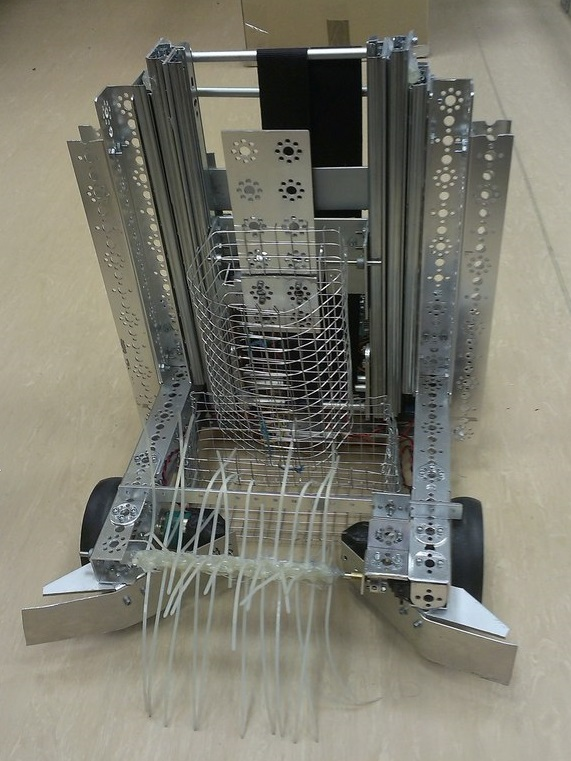
\includegraphics[scale=0.3]{days/16.11.14/images/01}}
				\caption{Bucket in a start position}
			\end{minipage}
			\hfill
			\begin{minipage}[h]{0.47\linewidth}
				\center{
\includegraphics[scale=0.25]{days/16.11.14/images/02}}
				\caption{Bucket in the overturned position}
			\end{minipage}
		\end{figure}
		
	\end{enumerate}
	
	\item Results:
	\begin{enumerate}
		\item Framework of bucket was created and installed to robot.
		
	\end{enumerate}
	
	\item Tasks for the next meetings:
	\begin{enumerate}
		\item To improve the bucket's construction.
		
		\item To test the bucket.
		
	\end{enumerate}     
\end{enumerate}
\fillpage

